% !TEX root = ../main.tex

\chapter{算法实现}
本文算法基于光滑自由变形\cite{Cui15},所以在变形、调整变形结果、绘制时所用的算法都与光滑自由变形相同。\autoref{fig:algorithm_ours}中是本文方法的流程图,可以与\autoref{fig:algorithm_sffd}对比发现,除了步骤3(切割三角形)采用了第\autoref{clip_algorithm}节中描述的算法,其它步骤均采用与光滑自由变形相同算法。

\begin{figure}
	\centering
    \tikzstyle{GPU} = [rectangle, draw, fill=blue!15, 
        text width=15em, text centered, rounded corners, minimum height=3em]
    
    \tikzstyle{CPU} = [rectangle, draw, fill=red!15, 
        text width=15em, text centered, rounded corners, minimum height=3em]
    \tikzstyle{line} = [draw, thick, ->, >= stealth]
    \begin{tikzpicture}[node distance = 2cm, auto]
        % Place nodes
        \node [CPU] (read) {1、输入多边形网格模型,并三角化};
        \node [CPU, below of=read] (initspace) {2、初始化B样条空间};
        \node [GPU, below of=initspace] (pntriangle) {3、求子三角面片的PN-Triangle,用以调整变形结果};
        \node [GPU, below of=pntriangle] (split) {4、用三角形均匀剖分算法分割三角形};
        \node [GPU, below of=split] (sample) {5、根据控制顶点,计算采样点的位置与法向};
        \node [GPU, below of=sample] (deformation) {6、用带约束的拟合的方法,计算出三角贝赛尔曲面片和法向量场的控制顶点};
        \node [GPU, below of=deformation] (adjust) {7、用法向信息和PN-Triangle信息调整上一步得到的控制顶点};
        \node [GPU, below of=adjust] (tess) {8、细分变形结果并绘制};
        \node [CPU, right=2em of deformation] (edit) {9、用户编辑控制顶点};

        % Draw edges
        \path [line] (read) -- (initspace);
        \path [line] (initspace) -- (pntriangle);
        \path [line] (pntriangle) -- (split);
        \path [line] (split) -- (sample);
        \path [line] (sample) -- (deformation);
        \path [line] (deformation) -- (adjust);
        \path [line] (adjust) -- (tess);
        \path [line] (tess) -| (edit);
        \path [line] (edit) |- (sample);
    \end{tikzpicture}
    \caption{本文算法流程图\\红色框表示在CPU中运行,蓝框表示在GPU中运行}\label{fig:algorithm_ours}
\end{figure}

本文以一个三维模型编辑器(如\autoref{fig:FFD_editor}所示)的形式实现我们的算法。程序整体用Python3.5实现,界面部分借助PyQT5\footnote{PyQT5是Python对QT的一个封装,方便程序员通过Python使用QT的各种功能。}。变形和绘制部分均通过PyOpenGL实现\footnote{与PyQT5类似,PyOpenGL是Python对OpenGL的封装},其中变形部分采用Compute Shader实现,绘制部分采用Rendering Shader实现。这两者可以访问到相同的内存空间,变形产生的输出可以直接作为绘制的输入,节省了变形与分制之间一次数据拷贝的开销。


\begin{figure}[htbp]
	\centering
	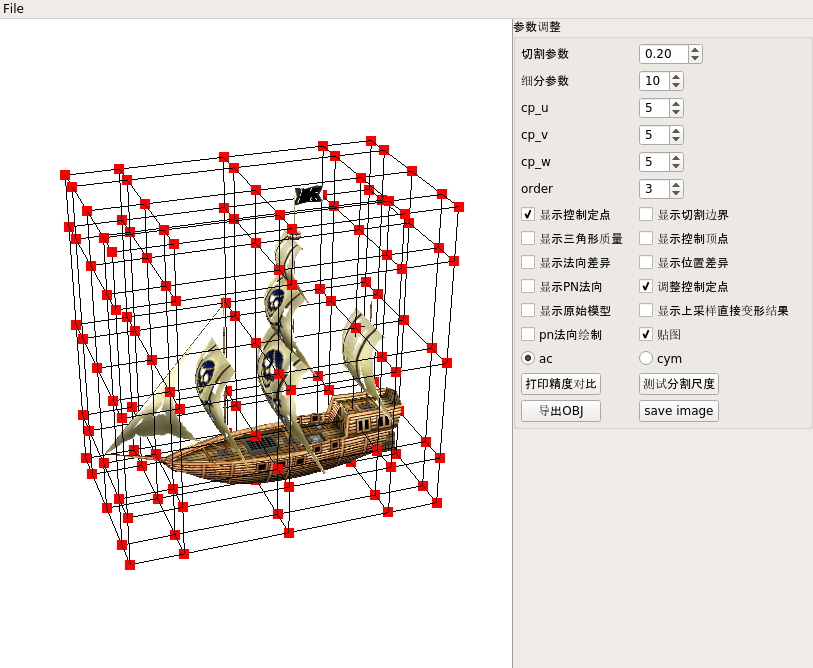
\includegraphics[width = 0.9\textwidth]{ffd_editor.png}
	\caption{三维模型编辑器}\label{fig:FFD_editor}
\end{figure}


\section{OpenGL Compute Shader实现}
CUDA是由英伟达公司推出的利用GPU进行并行通用计算的技术。该技术提供了方便易用的API,允许用户利用GPU强大的并行计算能力来加速算法,得到了学术界和工业界的广泛应用。光滑自由变形\cite{Cui15}基于CUDA实现。大概获得了100多倍的加速。但是CUDA只能的在英伟达的硬件设备上运行,这大大限制了光滑自由变形的通用性,光滑自由变形不仅无法应用在其它的桌面平台的GPU(AMD、Intel核显)中,也无法在移动平台中运行。而后者由于计算资源有限,反而更加依赖GPU加速算法。

为了使我们的算法更加通用,我们将原先在光滑自由变形中GPU加速相关的代码从CUDA迁移到了OpenGL Compute Shader,后者是OpenGL在4.3版本加入的一个新的着色器,主要用于GPU并行计算。由于OpenGL在每次调用图形相关API与GPU通信时,都会产生一定的开销,而将零散的GPU指令集中发送\footnote{即将多个绘图命令批量发送给GPU}可以提供给GPU更大的优化空间。所以我们将步骤5至步骤8实现在了同一个Compute Shader中\footnote{在Shader中,无法测量内部的某一段代码的运行时间,所以在\autoref{tab:deformation_time_compare}中,我们没能给出本文方法在变形相关的各个子阶段的运行时间,只给出了整个变形阶段所用的时间。},不妨称之为Deform Shader。算法通过步骤9读取用户输入,再由Deform Shader对模型进行变形。这两个过程交替进行,以达到实时编辑模型的目的。

但是生成PN-Triangle阶段和均匀剖分三角阶段实现在了两个不同的Shader中,因为我们在分割阶段需要邻接三角形的PN-Triangle信息,所以生成原始三角面片的PN-Triangle必需在均匀剖分原始三角面片之前进行。其中步骤3中产生的结果将会用于步骤8中,以调整控制顶点位置。步骤4用本文算法对原始三角面片进行剖分,主要目的是减少变形误差,提高变形结果的精度。


\section{三角均匀剖分算法的GPU实现}
    对比\autoref{tab:clip_time_compare}与\autoref{tab:deformation_time_compare}中光滑自由变形的运行时间可以发现,相对于变形过程所用的时间,按节点盒切割三角面片阶段所用时间非常久,比整个变形阶段慢了大约有100倍。虽然该过程只在模型载入阶段执行一次,但是过长的加载时间,仍会对用户体验造成影响。

    上述现象的原因在于光滑自由变形中,这一过程是在CPU中实现的。之所以不用GUDA,是因为分割过程中需要随机的引用不同的数据,且控制流程较为复杂,不适合在GPU中实现。

    本文分割方式也具有以上特点,除此之外,本文分割过程还是一个递归的算法,同样不适合在GPU中实现。为了使用GPU加速我们的分割算法,我们需要对均匀分割算法进行了一定的改进。

    首先,由于三角形均匀分割算法在计算三角形的某一条边需要被分成几段时,有一个取整操作。这就使得拥有不同但相近的边长的三角形,它们分割结果可能很相近,甚至一样。我们不妨将这些拥有相同分割方案的三角形称作“同类三角形”。同时,我们经过观察发现,对于同类三角形,可以共用一套分割方案,而不会引起子三角形质量的大幅下降。

    基于以上观察,我们将第\autoref{clip_algorithm}章分成了两个阶段:计算分割方案、应用分割方案剖分三角形。


    第一个阶段在CPU中进行,我们令$l=1$,然后计算边长为整数的、不同的三角形的分割方案,分割方案由两部分组成:子三角形的顶点在原三角形中的重心坐标、各个子三角形的顶点的连接关系。通过这些信息,可以方便的还原一个三角形剖分结果。

    计算分割方案需要较大的计算量以及复杂的分支判断,所以这部分计算在CPU中进行。又因为“同类三角形”的分割方案相同,所以这些分割方案可以提前预计算,以避免实际切割时重复计算。

    实际分割过程几乎不会将一条边分成20段以上,因为过多的三角形无法显著提高变形结果的精度,反而会影响程序效率。所以在这一过程中,我们计算了所有三边长为$\{len_i\}^{2}_{i=0}, len_i \in \mathbb{Z}, 1 <= len_i <= 30, len_0 + len_1 > len_2, |len_0 - len_1| < len_2$的三角形的分割方案\footnote{分割方案在整个软件生命周期中只需计算一次,而不是每次运行都要计算一次}。并将分割方案以$\{len_i\}^{2}_{i=0}$为索引存储到一张查找表中。


    第二个阶段在GPU中进行,先计算$\{\lceil len_i/l \rceil\}^{2}_{i=0}$,再以$\{\lceil len_i/l \rceil\}^{2}_{i=0}$为索引从查找表中找到分割方案,然后通过分割方案中分割点的重心坐标与原始三角面片的顶点位置为输入,用矩阵乘法直接求出分割点的位置。接着我们根据分割方案中的连接关系,构造出各个子三角形。上述过程没有递归,且分支较少,可以通过GPU并行计算架构获得较大的加速。

    实际上,我们是原从三角均匀剖分算法中,将“同类三角形”重复计算分割方案的过程提了出来。并与GPU中实际分割过程解耦。然后运用以空间换取时间的方法加速了分割过程。不仅如此,解耦后算法的复杂度集中在了第一阶段,使得第二阶段可以用GPU加速。所以本文的切割算法比光滑自由变形中的算法快了近200倍,如\autoref{tab:clip_time_compare}所示。

    但是在该算法中,“同类三角形”如果由原来的三角均匀剖分算法直接切割,所得到的子三角形并不一定相同,至少CVT优化后的结果会有所差别。所以该方法会使子三角形的质量略微下降,但是相比其带来的优势,我们仍有理由采用这一方法。
